% Section 3 - Real-Time Applications
% Roberto Masocco <roberto.masocco@uniroma2.it>
% Alessandro Tenaglia <alessandro.tenaglia@uniroma2.it>
% June 5, 2024

% ### Real Time Applications ###
\section{Real-Time Applications}
\graphicspath{{figs/section3/}}

% --- Real-Time Applications ---
\begin{frame}{Real-Time Applications}
		MARTe2 offers a generic base application, see \texttt{MARTeApp.cpp}.\\
    \bigskip
		Real-Time Applications are built (more like "bootstrapped" or "put together") from the base one through \textbg{configuration files} (\texttt{.cfg}).\\
    \bigskip
		The \textbg{configuration files} define all the software components of a RTApp and their configuration properties, \emph{e.g.}, the algorithms to be executed (\textbg{GAMs}) and the hardware or software modules involved (\textbg{Data Sources}).
\end{frame}

% --- Configuration file structure ---
\begin{frame}[fragile]{Configuration file: RTApp}
	\begin{columns}\column{.9\textwidth}
		\begin{lstlisting}[style=small, language=cfg, caption=RTApp high-level configuration structure.]
$RTApp = {
  Class = RealTimeApplication
  +Functions = { // GAMs
    Class = ReferenceContainer
    ...
  }
  +Data = { // Data Sources
    Class = ReferenceContainer
    ...
  }
  +States = { // RT States
    Class = ReferenceContainer
    ...
  }
  +Scheduler = { // Scheduler
    ...
  }
}\end{lstlisting}
	\end{columns}
\end{frame}

% --- GAMs ---
\begin{frame}{GAMs}
	\only<1,3>{
		\begin{block}{Generic Application Module}
			The \textbf{GAMs} are the software components where \textbf{real-time user algorithms} must be implemented.
		\end{block}
	}
	\only<2>{
		\begin{figure}
			\centering
			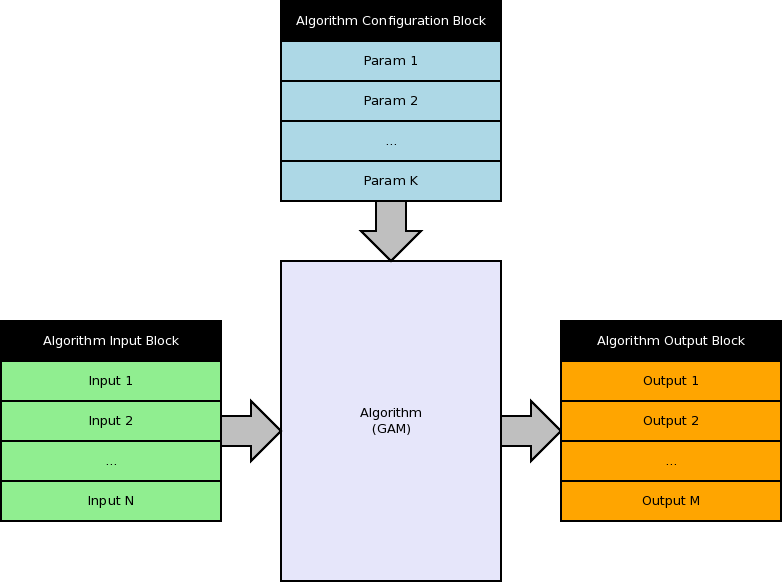
\includegraphics[scale=.3]{GAMs.png}
			\label{fig:gams}
			\caption{GAM operational scheme.}
		\end{figure}
	}
	\only<3>{
		\begin{alertblock}{}
      \centering
			\textbr{They should not perform neither data I/O operations nor OS calls\\(\emph{e.g.}, accessing files, network sockets, devices...).}
		\end{alertblock}
	}
\end{frame}

% --- Configuration file: GAM ---
\begin{frame}[fragile]{Configuration file: GAM}
	\begin{columns}\column{.8\textwidth}
		\begin{lstlisting}[style=small, language=cfg, caption=GAM configuration structure.]
+GAM1 = {
  Class = ExampleGAM
  InputSignals = {
    Input1 = {
      DataSource = DDB1
      Type = uint32
    }
  }
  OutputSignals = {
    Output1 = {
      DataSource = DDB1
      Type = uint32
    }
  }
  Parameters = {
	  Param1 = (uint32) 1000
  }
}\end{lstlisting}
	\end{columns}
\end{frame}

% --- DataSources & Brokers ---
\begin{frame}{DataSources \& Brokers}
	\begin{block}{DataSources}
		The \textbf{DataSources} are the software components that provide an interface for the \textbf{exchange of input and output signals data} with the memory and the hardware.
	\end{block}
	\begin{block}{Brokers}
		The \textbf{Brokers} are the software components that provide the \textbf{interface between the GAMs and the DataSources memory areas}, exchanging data between the two.
	\end{block}
  \bigskip
	\begin{figure}
		\centering
		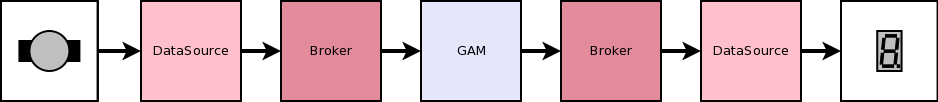
\includegraphics[scale=.35]{DataSources.png}
		\label{fig:datasources}
		\caption{DataSources and Brokers operational scheme.}
	\end{figure}
\end{frame}

% --- Configuration file: DataSource ---
\begin{frame}[fragile]{Configuration file: DataSource}
	\begin{columns}\column{.8\textwidth}
		\begin{lstlisting}[style=small, language=cfg, caption=DataSource configuration structure.]
+Data = { // Identifies DataSources section in the cfg
  Class = ReferenceContainer
  +DDB1 = {
    Class = GAMDataSource
  }
  +Timer = {
    Class = LinuxTimer
    SleepNature = Default
    Signals = {
      Counter = {
	    Type = uint32
	  }
      Time = {
        Type = uint32
      }
    }
  }
}\end{lstlisting}
	\end{columns}
\end{frame}

% --- States ---
\begin{frame}{States}
		\textbg{GAMs} are grouped in \textbg{real-time threads} which are executed in the context of specific \textbg{states}.\\
    \bigskip
		A Real-Time Application shall be in one (\textbg{and only one}) state at a given time.
\end{frame}

% --- Configuration file: States ---
\begin{frame}[fragile]{Configuration file: States}
	\begin{columns}\column{.8\textwidth}
		\begin{lstlisting}[style=small, language=cfg, caption=States section of a configuration file.]
+States = { // Identifies the States section
  Class = ReferenceContainer
  +State1 = { // For every state, multiple threads
    Class = RealTimeState
    +Threads = {
      Class = ReferenceContainer
      +Thread1 = {
        Class = RealTimeThread
        CPUs = 0x8 // CPU affinity
        Functions = {GAMTimer, ...} // Multiple GAMs
      }
      ...
    }
  }
  ...
}\end{lstlisting}
	\end{columns}
\end{frame}

% --- Configuration file: Scheduler ---
\begin{frame}[fragile]{Configuration file: Scheduler}
		A \textbg{real-time, OS-abstracting scheduler} handles the execution of real-time threads.
	\vspace{1cm}
	\begin{columns}\column{.8\textwidth}
		\begin{lstlisting}[style=normal, language=cfg, caption=Scheduler section of a configuration file.]
+Scheduler = { // Identifies the Scheduler section
  Class = GAMScheduler
  TimingDataSource = Timings
}\end{lstlisting}
	\end{columns}
\end{frame}

% --- Example: Real-Time Application  ---
\begin{frame}{Example: Real-Time Application}
	\begin{figure}
		\centering
		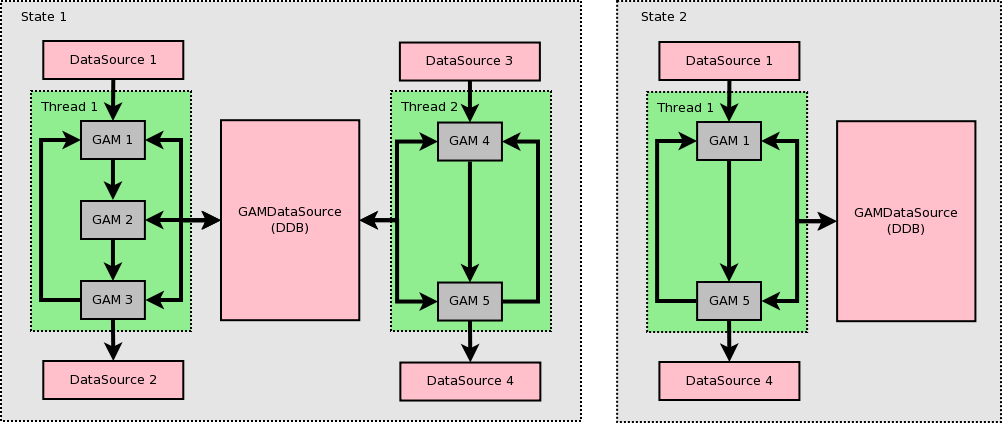
\includegraphics[width=.95\textwidth]{RTApp.png}
		\label{fig:rtapp_example}
		\caption{Example of a multi-state and multi-threaded Real-Time Application.}
	\end{figure}
\end{frame}
